\documentclass[conference]{IEEEtran}
\pdfpagewidth=8.5in
\pdfpageheight=11in
%\usepackage{subfig}
\usepackage{subfigure}
%\usepackage{extsizes}
%\usepackage{subcaption}
\usepackage[pdftex]{}
\usepackage{graphicx}
%\usepackage{todonotes}
\usepackage{listings}
%\usepackage{hyperref}
\usepackage[breaklinks,colorlinks]{hyperref}
\usepackage{url}
\usepackage{todonotes}
\usepackage{amssymb}
\usepackage{xspace}
\usepackage[binary-units=true]{siunitx}

\lstset {% general command to set parameter(s)
  language=C,
  basicstyle=\footnotesize,               % print whole listing small
  %     keywordstyle=\color{black}\bfseries, % underlined bold black keywords
  %     identifierstyle =\color{black},  % nothing happens
  %     commentstyle=\color{black}\emph, % white comments
  %stringstyle=\ttfamily,          % typewriter type for strings
  %     stringstyle=\color{black},       % typewriter type for strings
  tabsize=4,
  showtabs=false,
  showstringspaces=false}
%can't figure this one out for particles bandwidth
%\usepackage[caption,label]{subfig}
\def\Snospace~{\S{}}
\renewcommand*\sectionautorefname{\Snospace}
\def\sectionautorefname{\Snospace}
\def\subsectionautorefname{\Snospace}
\def\subsubsectionautorefname{\Snospace}
\newcommand{\MB}{\,\text{MB}\xspace}
\newcommand{\GB}{\,\text{GB}\xspace}
\newcommand{\ada}[1]{\textcolor{red}{Ada: #1}}
\newcommand{\DDT}{D\textsuperscript{2}T~}
\newcommand{\DDTns}{D\textsuperscript{2}T}
\newcommand{\subsubsubsection}{\noindent\textbf}
\newcommand*{\captionsource}[2]{%
  \caption[{#1}]{%
    #1%
    \\\hspace{\linewidth}%
    \textbf{Source:} #2%
  }%
}
%\addtolength{\parskip}{-0.08in}

% in order for balance columns to work, it has to be before begin document...
%\balancecolumns

\begin{document}

\title{SuperGlue: Tradeoffs and Tipping Points for Extreme Scale Workflows}

\author{
  \IEEEauthorblockN{
Alexis Champsaur\IEEEauthorrefmark{1},
Jay Lofstead\IEEEauthorrefmark{2},
Jai Dayal\IEEEauthorrefmark{1},
Matthew Wolf\IEEEauthorrefmark{1},\\
Greg Eisenhauer\IEEEauthorrefmark{1},
Ada Gavrilovska\IEEEauthorrefmark{1},
Matthieu Dreher\IEEEauthorrefmark{3},
Tom Peterka\IEEEauthorrefmark{3}
}
  \IEEEauthorblockA{
\IEEEauthorrefmark{1}School of Computer Science, Georgia Tech,
\IEEEauthorrefmark{2}Sandia National Laboratories,
\IEEEauthorrefmark{3}Argonne National Laboratory
}
}

\maketitle

\begin{abstract}


Multi-step scientific workflows have become prominent and powerful tools of
data-driven scientific discovery. Run-time analytic techniques are now commonly
used to mitigate the performance effects of using parallel file systems as
staging areas during workflow execution. However, workflow construction and
deployment for extreme-scale computing is still largely an \textit{ad hoc}
process with uneven support from existing tools. In this paper, we present \sys,
an approach to designing generic, reusable components for end-to-end construction
of workflows. Specifically, we demonstrate that a small set of \sys generic components
can be reused to build a diverse set of workflows, using examples based on actual analytic
processes used in three well-known scientific codes. Our evaluation shows
promising scaling properties, as well as
negligible overheads for using a modular approach over a custom, ``all-in-one''
solution.  As extreme-scale systems become
increasingly used for data analysis as well as simulation, tools such as \sys
will become increasingly valuable for defining and deploying flexible, efficient
workflows.


\if 0
Scientific simulation workflows have traditionally used the storage array as a
staging place between the components that make up the workflows and employed a
high-level task manager to trigger these components.
Recent work has been investigating moving
these workflows to purely online models, thus avoiding the well-known
performance bottleneck of storage arrays.  One key advantage of moving to a
purely online model is the ability to launch the entire workflow as part of a
single submission, thus avoiding
the challenges that existing workflow management systems face
in launching individual components on HPC platforms. Still, there lacks
a generic way to assemble complete workflows, even with
many workflows using similar analytical routines.

In this work, we present Superglue, an approach for
assembling entire workflows from existing components
and submitting workflows as single jobs, all through
a single job submission shell script.
We leverage the self-describing, process size- and placement-independent
properties of data exchanged by the Adaptable I/O System (ADIOS) as well as the
MxN publish-subscribe model of Flexpath to assemble and run three Superglue
workflows based on three different and widely-used simulation codes exporting
different data formats.  We show that the performance cost of a componentized
approach to assembling workflows is small, especially when considering the
ability to assemble complete workflows ``out of the box.'' While keeping in
mind performance considerations, we present the building blocks as well as an
approach to expand a library of such components, which we hope can eventually
meet a wide variety of analytical needs in the scientific computing community,
in the common scenario of submitting a workflow as a single job to a
supercomputer scheduler.
\fi

\end{abstract}

\if 0
The workflows are assembled using
some of the same components, but leading to very different analytical results.
In this way, we present the building blocks of a library of generic components


Scientific simulation workflows are becoming a 
Considering the well-known bottleneck that is the persistent storage array,


Scientific simulation workflows have traditionally focused on using the storage
array as a staging place between components and employ a high level task
manaager to trigger components. Recent work has been investigating moving these
workflows to purely online models avoiding the storage array bottlenecks. This
transition is not cost free, but there are also potentially enormous advantages.
For example, by moving online, more the data movement is limited by bisection
bandwidth rather than storage bandwidth. However, making existing tools work
online may take some modification and adding in the ``glue'' components required
to translate the output from one component to the input for the next are no
longer simple scripts.

This paper examines these tradeoffs and lays out when the advantages may make
moving purely online worthwhile even though not being forced by platform
limitations. Support tools necessary to support both models are also discussed
including offering standardized ``glue'' components for online workflows making
the transition easier.
\fi


%\category{D.4}{Software}{Operating Systems}
%\category{D.4.7}{Operating Systems}{Organization and Design}[hierarchical design]

%\terms{Design, Performance}

\section{Introduction}
\label{s:intro}

As extreme computing architectures continue to evolve, it is 
clear that I/O is an increasingly significant problem.  Projections suggest no
significant parallel file system I/O bandwidth growth through the next 100x
increase in compute capabilities.  The traditional HPC approach of writing
complete checkpoints or analysis dumps for later processing to gain scientific
insights is becoming infeasible.  Even with technologies like Burst Buffers,
limited capacity reduces the usefulness. As such, in situ and in transit
analysis and visualization toolkits with the capability to reduce, process, and
otherwise mitigate the raw increase in data volume and throughput requirements
are increasingly important.

% here we go directly from in situ argument
% to examples of workflows. needs transition. ok.
% also, confusing to go into detail about the existing
% WMSs here and then have a related work section.
% reduce.

Scientific workflows, which 
capture a series of such analytical steps for a
particular scientific discovery goal, usually
by operating on large quantities of data,
have also followed this trend of moving the analytical components
online (ie. executing simultaneously with the driving scientific code).
A number of scientific workflow engines exist.
However, while workflow engines such as
Kepler~\cite{bertram:2006:kepler} and
DAGMan~\cite{Malewicz:2006:dagman}
offer flexible ways to assemble components
with rich functionality to manage the control flow, they have not been
universally adopted due to some of their limitations and complexity in the
HPC environment.

An example illustrating the complexities comes from the Oak Ridge
Leadership Computing Facility (OLCF).  Kepler was used for several workflows
for the fusion simulation users.  While the initial goal was that an internal,
expert resource would create the workflow,
including the data transformation code required
to allow downstream components to operate on the output of
uptream ones (ie. the ``glue code''),
the workflow should be able to be maintained
easily by the application scientists. Unfortunately,
the expert was required regularly as the configuration evolved and scaled.
The complexities of maintaining the components and the glue code as the output
shifted and managing the deployment was too high.
Even then, the workflow operated offline.

One major limitation to existing workflow engines is that
given only a simluation code, a scientist cannot easily
assemble a workflow ``out of the box.''
Indeed, even with the re-use of code that performs
common analytical procedures and with the automation of control flow
allowed by existing engines,
for a scientist to assemble
and launch a workflow using existing tools,
significant effort is required to (a) allow the existing
analytics code
to operate on the specific data formats used in this
particular workflow,
(b) reconcile the discrepancy between the potentially
differing levels of parallelism
of the various components,
and (c) map the workflow components
to the available resources, which in the HPC space
is usually a supercomputer.

% I see a, b, and c as the main problems we are solving with SG
% -> (a) with the any-dimension genericity of tools like select and dim-reduce
% -> (b) with the use of a simple bash script to launch a full workflow, which is
% a common scenario
% -> (c) by the automatic partitioning of data that the components do,
%        without special knowledge required from the scientist.


%not sure where this fits, but not here
\if 0
Distributed-Area Computing
(DAC) workflow management
systems~\cite{tejedor:2015:pycompss,deelman:2015:pegasus} and HPC workflow
management systems~\cite{dorier:2015:in-situ-lessons} may need to interoperate
for some scenarios~\cite{deelman:2015:workflows-report}. While both exist, to
date they have been developed separately in different communities. We have only
just recently begun to develop a plan and a prototype for integrating such
heterogeneous workflow systems. This paper focuses on managing the HPC portion of
these heterogeneous workflows.
\fi

%Figure 1 is an example of such an integration.  It shows a top level
%DAC workflow with one of the nodes in the DAC workflow graph being an HPC
%workflow graph running on a supercomputing center. The interfaces between the
%two WMSs occur from DAC to HPC and from HPC to DAC. The former interface
%requires the exchange of the HPC subworkflow graph, which presumably was
%defined by the user through the interaction with the top-level DAC WMS, and the
%exchange of data products produced by the DAC that need to be further processed
%by the HPC subworkflow. The latter interface, from HPC to DAC, involves the
%transfer of data products only.

% we already talked about the trend of moving workflows online
\if 0
Falling back to Python
scripts managed by the application scientist proved easier and faster to
maintain. While this approach using the parallel file system to stage
intermediate data was sufficient, it is quickly becoming infeasible. The IO
overhead for using the parallel file system is exceeding acceptable runtime
percentages forcing a reduction in output and making scientific insights more
difficult to discover. 
\fi

Proposed infrastructure for online workflows is less mature but can offer
the necessary functionality for assembling workflows
ad-hoc~\cite{zheng:2010:predata,docan:2010:dataspaces,wolf:2002:smartpointer,abbasi:2009:datastager}.
For example, in PreDatA~\cite{zheng:2010:predata}, separate applications are
run to offer different resilience domains, but the actual placement of
operators may be different depending on the performance characteristics requiring
coding changes for each placement decision.
DataSpaces~\cite{docan:2010:dataspaces} offers a way to map data from one
application to another, but it has no mechanisms to manage what is a complete
data set, when it begins in an output stream, and when it ends. The user has to
determine if what is being requested is complete and correct or not.
Data Staging~\cite{nisar:2008:staging} and in particular
data staging with processing
capabilities~\cite{abbasi:2009:datastager,ober:seismic}, are a solid step
forward in providing online functionality for workflows, but do not 
offer a generic approach for their assembly.
SmartPointer~\cite{wolf:2002:smartpointer} and
DataStager~\cite{abbasi:2009:datastager} both offer examples of integrated
workflows, but the construction is completely custom and not portable to other
workflows.

%\ada{this is a very vague claim, doesn't help explain the key
%  problem. the previous paragraph above is, is there more evidence?}

This lack of a robust infrastructure and the difficulty in
using these tools direcly to assemble an
HPC workflow out of the box
based on an existing scientific code,
simulation or other,
and launching it in a way that is
as simple as a single job submission
have limited their adoption.

Newer work is extending these
systems to provide more generic functionality
in workflow assembly and
management~\cite{dayal:2014:flexpath,dayal:2015:escience,lofstead:2012:txn,lofstead:2013:txn-pdsw,lofstead:2012:txn-metadata,lofstead:2014:txn,lofstead:2016:superglue}.
In particular, FlexPath~\cite{dayal:2014:flexpath}
is a publish/subscribe system that allows
two concurrently running MPI executables to
exchange data that is globally partitioned among
their ranks, even when the number of writers and readers differ.
It is implemented as a transport method for the
Adaptable I/O System (ADIOS)~\cite{lofstead:2009:adaptable},
which provides a unified interface to parallel I/O over a rich
variety of underlying data encoding, transport, and placement technologies.
With ADIOS, FlexPath provides a simple interface for MxN communication
between simulation and/or analytical components.
Through ADIOS and FlexPath, data exchange makes use
of the abstraction of a stream, which allows
for asynchronous, MxN I/O between workflow components.

In this work, we leverage the stream-based, MxN
I/O interface offered by ADIOS and FlexPath
to present SuperGlue, a collection of generic workflow components
that allow for the easy assembly and deployment
of a variety of scientific workflows.

SuperGlue allows workflows to be assembled
by using existing, generic
data transformation and 
analysis components
which to not require any code changes
for specific workflows;
the only code changes required when
using SuperGlue are 
for redirecting of the output of interest
in the driving simulation code through ADIOS.

SuperGlue components solves a number of the aforementioned problems in
current online workflow-oriented technologies.
First, they leverage the self-describing
property of data exchanged through ADIOS to
allow for operation on data having very different formats.
In scientific workflows, the data of interest
is generally composed of large, multi-dimensional
arrays; in SuperGlue, this translates to
the ability to operate, as much as possible,
on data having any number of dimensions.
To address the difficulty and complexity
in mapping workflows to supercomputers using
existing workflow technology, which is targeted
at a variety of resources outside of HPC, such as Grid and Web
resources,
SuperGlue reduces the
launch of an entire workflow to the submission of a single job script.
Finally, it uses the MxN publish/subscribe
ability of FlexPath,
as well as consistent semantics describing
the data that are passed through the components,
to exchange data while preserving semantic integrity
even in the presence of varying levels of parallelism 
at different stages of the workflow.

Rather than providing a complete collection of such components,
we provide here the basic building
blocks of what we hope will be a library of components that can
eventually be used to assemble
a rich variety of workflows, driven by simulation codes
exporting a variety of different data formats.

\ada{sell the work. highlight something that says: your contributions are the design (you thought
  about what's the right lower level functionality you can leverage to
  make this work), collection of generic SG filters, and demonstration
through large-scale deployment of three different workloads that the
approach is 
expressiveness, can impact productivity since components can be reused
with minimal intervention, and doesn't impeed performance and
experimentation at scale. }
To demonstrate the functionality of the SuperGlue approach,
deploy three SuperGlue workflows based on three different
scientific simulations having large user bases,
namely the LAMMPS molecular dynamics simulator~\cite{plimpton:1997:lammps},
GTCP, a particle-in-cell toroidal plasma code~\cite{lin:gtc},
and GROMACS, a biochemical molecular dynamics code\cite{hess2008gromacs}.
We show that SuperGlue allows workflows to scale well and that
simple experiments allow for the selection of
appropriate levels of parallelism at different
stages of the workflow.

One disadvantage that might be perceived in the fine-grain componentization
of a workflow that naturally comes with the use of SuperGlue
is the potential loss in performance.
However, we show through a performance comparison of
a componentized, generic workflow with a corresponding
ad-hoc workflow which uses a monolithic analytical component
that the componentization of analytical routines
does not lead to a noticeable change in the
overall performance of the workflow.

%While the online shows a lot of potential to improve the scientific discovery
%process, it requires reworking existing workflows. Since this is a non-trivial
%task, tools that can simplify creating an efficient workflow within a single job
%submission is crucial to adoption.
%\ada{text before not clear}
%New workflows can
%be made from scratch online lowering the barrier, but there are still costs
%associated with using existing components that may or may not integrate well
%into the online structure.

%The ``killer app'' for workflows, both offline and online, is being able to
%submit a single job that is capable of running the entire workflow. Existing
%techniques to make this work requires machine reservations or special
%permission for automated connections between the management machine and the
%large scale platform.  SuperGlue's approach bridges the connectivity problems
%and addresses the data type mismatches common when data flows from one
%component to the next.

%========================

\if 0
To address the performance mismatch, Integrated Application Workflows (IAWs)
are being developed. The easiest way to think of these IAWs is the Unix/Linux
shell pipe operator to connect commands. The shell connects stdout of one
program to stdin of the next with the assumption that each component in the
chain can operate in this mode. For tasks at this scale, this approach works
well. For the scientific workflows we are targeting, we have processes spread
across potentially 10,000s of nodes connected to other components also running
on multiple nodes. Unlike the command-line tools, none of these components
generally have the ability to shift their input or output from how it is
written to connect to a new online component without potentially significant
code changes. The challenge with these workflows is dealing with the lack of a
persistent store to stage intermediate data, interfaces for communicating data
state and availability, and data organization changes required before a
component can process data.  Each of these has been investigated by different
projects over the last several years.

Several frameworks have been developed that offer some functionality for
supporting online workflows. The more advanced examples incorporate some data
processing components, sometimes of limited scope, for performing in situ or in
transit processing. The ADIOS IO library~\cite{lofstead:2009:adaptable} was designed with
this use case in mind. The HDF5 Virtual Object Layer
(VOL)~\cite{chaarawi:2013:hdf5-vol} was developed to support similar
functionality.

Several efforts to work through some of the issues related to IAWs have been
investigated~\cite{karimabadi:2013:catalyst,whitlock:2011:libsim,Glean,dayal:2014:flexpath,dreher:2016:bredala,zheng:2010:predata},
and much on-going research in the space promises to expand on some of the
needed techniques for management and placement.  Some
scientific codes have been addressing similar constraints for years by
in-lining analytics functions and performing complicated MPI communicator
subdivisions to allow simulation and analytics to co-exist.  One key
observation, however, is that there is a lack of portability to the resulting
implementations; they require a great deal of tuning and/or runtime placement
control to make them function as desired.
\fi


\if 0
Unlike existing components used in IAWs, SuperGlue
components do not have a fixed data type. \ada{if this is the key
  difference, then somewhere mention the fixed type limitation. }
 This one change enables using these
components on completely different kinds of simulations that share nothing in
their output format. Key to making this work is using a typed transport
mechanism between different components. Many options exist for these transports
and the particular mechanism selected is not critical. 

\ada{summarize some insight here: what do you leverage/need in order
  to be able to templetize the glue components, and then to permit the
same approach to work for instantiating analytics... typed transport
is one, anything else?}
In an effort to better understand when choosing one approach for constructing a
workflow is perferable to another, we have developed a collection of ``filters''
we call SuperGlue that allow us to experiment with the tradeoffs. This paper
describes our components and examines some different workflows constructed using
different techniques to compare when the costs and benefits for one approach are
a better tradeoff than for others. 
\ada{sell the work. highlight something that says: your contributions are the design (you thought
  about what's the right lower level functionality you can leverage to
  make this work), collection of generic SG filters, and demonstration
through large-scale deployment of three different workloads that the
approach is 
expressiveness, can impact productivity since components can be reused
with minimal intervention, and doesn't impeed performance and
experimentation at scale. }
Our main contribution is the evaluation of
these workflows constructed using different engines and techniques to understand
when different approaches become viable, such as IAWs, or if cobbling something
together is sufficient or even superior for certain metrics.
%analysis and manipulation tools that can be chained together to form a variety
%of real-time workflows providing analytical results during the execution of the
%primary scientific code.

While the main technical development contribution of this work is the design of
generic {\em glue code}, the {\em analytical} components we use in the
workflows we present here are designed using the same approach. For example, an
index selection tool is more of a glue component while a histogram component is
more analytical.  Still, we design both types of components as single MPI
executables with similar input and output interfaces launched using similar
configuration options.  By blurring the line between generic glue components
and generic analytical components, we present a flexible way to assemble
scientific workflows without having to write any additional code. 
\fi

The rest of the paper is organized as follows. First is a survey or related
work in~\autoref{s:related}. Second, in~\autoref{s:workflow}, is a
discussion of the three workflows we use to drive our insights. Next is an
overview of the concepts behind SuperGlue in~\autoref{s:design}.
In~\autoref{s:reusable-components}, we provide an overview of the reusable
components created. In~\autoref{s:integrating-reusable-components}, we
discuss the challenges of integrating reusable components.  An evaluation is
presented next in~\autoref{s:eval}. Finally is a discussion of Conclusions
and Future Work in~\autoref{s:conclusion}.

\section{Related Work}
\label{s:related}

Existing workflow systems have typically only been able to offer generic,
reusable components when the workflow system is for a particular niche with a
fixed datatype and standardized interfaces. For example, enterprise document
processing systems may all work against a single database with each user only
seeing their current worklist. As documents are processed, they are moved to
the next work queue, or completed state, according to hand-coded
rules~\cite{mckesson-workflow}. The Workflow Management Coalition~\cite{wfmc}
has developed standards to make enterprise process workflows more portable.
These standards are not intended to make components reusable, but to make
different workflow engines able to inter-operate or to port a workflow from one
engine to another.  The actual communication interfaces and data types are left
to the components themselves.

More directly related to this work and the scientific community are workflow
engines and frameworks custom-made for the parallel computing environment.
Pegasus~\cite{mullender:pegasus} and DAGMan~\cite{Malewicz:2006:dagman} work
together to offer an engine to execute a workflow and a front-end system to
construct the workflow process itself.
However, the focus in DAGMan is on specifying dependencies between
the jobs involved in the workflow, so as to execute
components only when required and provide resilience.
In contrast, in SuperGlue, the entire workflow is executed at once, with
FlexPath allowing readers and writers to block until
the corresponding writer or reader is available for data exchange.
Furthermore, the Pegasus/DAGMan engine does not provide
a library of generic, reusable components.

As an alternative to DAGMan, Swift~\cite{wilde2011swift}
is a scripting language that allows ordinary applications
to be composed into parallel scripts, and eventually into
workflows, with dependencies specified in the script.
However, these applications themselves
must be written outside of the Swift script.

Kepler~\cite{bertram:2006:kepler} offers a nice GUI for assembling different
kinds of scientific workflows. It offers different directors to manage how the
workflow will be executed. Each component is an actor with channels connecting
actors. As mentioned in the Introduction, complex workflows using Kepler have been
assembled for many communities, including fusion science.
However, the variety of components
that come with Kepler are designed
to work in a single Java Virtual Machine instance;
using HPC-scale components requires significant effort
both in coding the custom components and in
allowing the I/O methods used to be understood by the Kepler engine.

To address much of the complexity of communicating between separate parallel
components, in situ approaches are being investigated.
We use ``in situ'' in the sense of ``linked into the same process.''
Catalyst~\cite{karimabadi:2013:catalyst} offers a way to integrate the
ParaView~\cite{Moreland:2008:paraview} analysis and visualization system
directly into the simulation executable. Catalyst strips out many features to
reduce the memory footprint and then requires explicit calls from the host
application into Catalyst routines with predictable data types on in-memory
data structures. While this can work for limited kinds of data processing,
it clearly cannot take advantage of additional resources
available for off-site analysis, instead taking cycles
away from the main scientific code.

%above is obvious enough I think
\if 0
two
limitations can cause problems. First, in an internal Sandia project in 2012,
the CTH shock physics code used ParaView both in situ and also in transit. The
in situ integration saw the executable grow from 30 MB to 300 MB and the
scalability was strictly limited due to design flaws in ParaView for in situ
use. While this project prompted the creation of Catalyst, this stripped down
version of ParaView does not address all concerns. There is still a memory
footprint overhead and a runtime pause in the simulation progress for the
analysis and visualization to run.
\fi

Libsim~\cite{whitlock:2011:libsim} has a similar relationship to
VisIt~\cite{Riedel:2007:visit} as Catalyst has to ParaView. Both Libsim and
Catalyst have a strict limitation that offline workflows do not. In both cases,
because they are running on the same nodes as the simulation, time series
analysis and visualization can be difficult or impossible. The potential
scaling impact on the simulation because of limitations in Libsim or Catalyst
can prevent their use for the most important use cases at extreme scale.

A middle path between in situ and offline processing was investigated in
PreDatA~\cite{zheng:2010:predata}.
This work demonstrates that the placement of the analytics can significantly
affect the performance of workflows, and that this placement can be determined
in part by the communication characteristics of the analytics components.

Glean~\cite{vishwanath:2011:glean}, Nessie~\cite{oldfield:lwfs-data-movement},
and Mercury~\cite{Soumagne:2013:mercury} are intended to facilitate offering
portable workflows across different interconnect technologies. While their
origins may not have been directly for addressing workflows, they have been
re-purposed to address this field. Rather than offering anything related to
managing data types, these tools simply offer a portable way to construct
workflows.

Companion work to SuperGlue within this same project is
Bredala~\cite{dreher:2016:bredala}. This work presents an attempt to build a
data model for in situ workflows. It has some similarity to
FFS~\cite{eisenhauer:2011:ffs}. Unlike FFS, which is part of a much more
complex infrastructure for typed messaging between distributed processes,
Bredala is strictly focusing on the data model.

Overall, while all of these efforts are addressing different portions of the
online workflows puzzle, none of them are addressing the idea of general,
reusable glue and analytical components for scientific workflows.

\section{Workflows}
\label{s:workflow}

We designed and implemented two realistic real-time workflows based on
scientific codes having large user bases: the LAMMPS Newtonian particle
simulator~\cite{plimpton:1997:lammps} and GTCP, a particle-in-cell Tokamak
simulator~\cite{lin:gtc}. While both of these workflows eventually turn the
simulation data into histograms of certain quantities of interest, how they
arrive at their final result varies significantly. Creating similar types of
results, and this using some of the same components but in significantly
different ways, has allowed us to gain important insight into how best to
design glue components that can be used in a wide variety of workflows.
We first describe the workflows from a general point of view
and then the components in greater detail, illustrated
in~\autoref{fig:lammps-workflow} and~\autoref{fig:gtcp-workflow}.

\subsection{LAMMPS Workflow}

We configure LAMMPS to simulate a disruption (a ``crack'') in a thin layer of
particles and output 5 numerical properties describing each particle in the
simulation at regular timestep intervals. This corresponds to two-dimensional
data (particles as one dimension and properties of interest as another) and
among these properties are the three-dimensional components of the particles'
velocities. In this case, the workflow outputs one histogram per timestep
showing the velocity distribution for all simulation particles at that point in
time.  From the LAMMPS output, the particular quantities of interest must be
extracted and then a histogram generated.

\subsection{GTCP Workflow}

\begin{figure}
  \centering
  \vspace{-0.10in}
  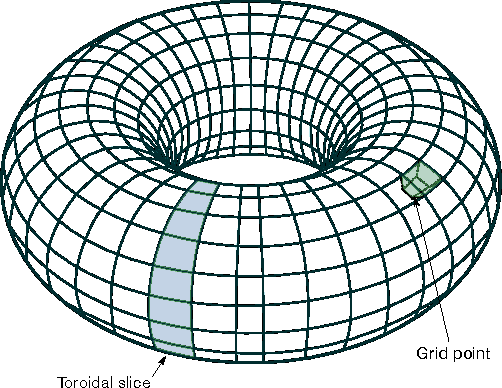
\includegraphics[width=0.7\columnwidth]{fig/Simple_Torus_mod}
  \vspace{-0.09in}
  \caption{Representation of GTCP Toroid, modification of \cite{WikimediaCommons:torus}}
  \label{fig:toroid}
  \vspace{-0.20in}
\end{figure}

GTCP, a code that simulates a toroidally confined plasma, splits the solid into
toroidal slices, each made up of a number of grid points. For each of these
grid points, it outputs 7 properties of the plasma such as pressure and energy
flux. This division of the toroid is illustrated in~\autoref{fig:toroid}.
The output of the simulation is therefore a three-dimensional array in which
the dimensions span: (a) toroidal ranks (toroidal slice number), (b) grid point
numbers, and (c) property indices. In this workflow, the per-timestep histogram
generated shows the distribution of per-gridpoint parallel pressure across
the entire simulation. From GTCP's output, the particular quantities of
interest must be extracted and then a histogram generated.

\subsection{Discussion}

In both cases, a particular subset of interest is extracted from the
output data set, a calculation is performed, and a histogram is
generated. This is illustrated in~\autoref{fig:generic-workflow}. In many
cases, the histogram component may be some standard, reusable operator.
The challenge is the data selection and mathematical
manipulation to obtain the quantities of interest in a way that (a) presents an
intuitive interface to the scientist constructing the workflow and (b) is
useful in different types of workflows in which data have different sizes and
dimensions.  This difficulty arises because (a) the data at each stage of the
workflow is distributed over the collection of processes involved in each
component even if it forms a coherent whole and (b) the extraction and
re-arrangement of multi-dimensional, distributed data, in a way that is
configurable by the user at runtime is challenging.  Both workflows are
similar, insofar as both codes generate a large output while we are only
interested in a per-timestep histogram of a particular simulation quantity.
However, because the simulations generate very different data, selecting the
relevant data from the simulations and formatting it in a such a way that the
final Histogram component can operate on it is done very differently in each
workflow.

\begin{figure}[htbp]
  \vspace{-0.1in}
  \centering
  \includegraphics[width=0.7\columnwidth]{fig/gwflow}
  \vspace{-0.09in}
  \caption{Generic Workflow Illustration}
  \label{fig:generic-workflow}
  \vspace{-0.10in}
\end{figure}

In typical scientific workflows today, custom glue code is written for
selecting relevant data and writing it so the ``formatter'' illustrated in~\autoref{fig:generic-workflow} can work.  Then, potentially additional
custom glue code will fix the histogram calculation into something that can be
rendered or saved as desired.  In this work, we demonstrate general, reusable
components capable of handling all three intermediate operations.

The workflows presented here use no custom glue code. Instead, the glue is
designed as generic components that accept command-line configuration options
at launch time. At most, the user specifies a few parameters and organizes
the components into a proper pipeline. Both of these operations are easy enough
that a non-expert
%application scientist
can create workflows through GUIs or other guided assembly techniques.

That we are able to use some of the same glue code to connect the start to the
end of each workflow shows that generic glue code that can manipulate large
datasets in real time is possible and useful for assembling very different
workflows.  In addition, we later show that generic components, both glue and
analytical, have the advantage of possessing known performance characteristics,
which greatly facilitates the configuration of workflows that use them.

\section{Design}
\label{s:design}

In this work, we offer some insight in the design of generic data manipulation
and analysis components from our implementation of two workflows. These
workflows are driven by two different scientific codes, yet they share some of
the same components. First, we present our insights and then discuss our
implementation choices and how they affect the project.

\subsection{Insights: Overview}

By evaluating the presented workflows and considering other workflows with
which the authors are familiar, four particular insights are revealed.

1) To allow for the greatest variety of workflows, data manipulation
  primitives and data analysis components should be packaged in similar ways --
  that is, regardless of their individual complexity, the pieces that make up
  these workflows should export compatible interfaces as much as possible.

2) The ability to handle multi-dimensional data, along with the consistent
  labeling of dimensions and quantities as meta-data, allows for components that
  are highly adaptable and simple to use.

3) While different types of components understand varying levels of
  semantics, maintaining a high level of semantics (i.e., labeling quantities and
  dimensions as much as possible) early on and when passing through components
  that do not necessarily require all of these labels allows for the most
  functionality downstream.

4) Because programming languages understand multi-dimensional data as being
  in a specific order in memory, there is a need for glue components that re-arrange
  data and re-label its dimensions without necessarily changing its size. Indeed,
  when data is stored in a database on disk, it is simple to gain a desired
  view of the data, for example by using SQL. However, in the middle of a
  real-time workflow, data must be presented to the components in a format that
  they expect and understand. This requires a specific ordering of
  data in memory. We expand on this topic
  in~\autoref{subsec:dimreduce}.

These insights guide the design for the reusable glue and analysis
components presented in this
paper. From a general perspective, designing a smaller number of
components to assemble workflows with finer step decomposition
allows for more general processing and more accurate performance
expectations than designing more numerous components each having more
complex functionality.

\subsection{Multi-Dimensional Data Support}

Many scientific codes serialize their output, effectively packing
multi-dimensional data into a single dimension. However, this technique offers
little information on the data to downstream components in a workflow.

For example, both of the simulations used in the workflows presented in this work
pack their output into one-dimensional arrays, even
though the output LAMMPS is logically two-dimensional, and that
of GTCP three-dimensional.
In order to use the same glue code to extract desired data from both outputs,
this code must be able to operate on two-dimensional data
as well as three-dimensional data. In fact, if the glue code is able to operate
on any number of dimensions, all that must be provided to it
at runtime is the
dimensions and indices to extract. This is precisely the role of our
{\em Select} component.

In general, it is advantageous to (1) design components that can operate on
multi-dimensional data as much as possible, and (2) format the output data of
scientific applications as having well-defined dimensions. Emphasizing the
support for multi-dimensional data in the design of workflow components allows
for maximum compatibility between the interfaces of components by providing a
consistent way to refer to the data.

Still, while multi-dimensional data support provides a consistent way to refer
to the data, not all components should be designed so as to work with
\textbf{\em any number} of dimensions. For example, we found it advantageous to
design our {\em Histogram} component to work with only one dimension.
Indeed, creating a histogram from one-dimensional data is intuitive.
Supporting a higher number of dimensions would add unnecessary complexity
to this component. If the data has more dimensions than are expected,
and only particular indices in a particular dimension hold the data of interest,
we can simply use filter and selector glue to extract and format the data for
{\em Histogram} to operate on.


\subsection{Semantics}

When data is organized under clearly defined dimensions, labeling these
dimensions and the indices they hold
as the data goes through each component lets downstream subscribers
refer to dimensions using their names. Because the data is potentially re-sized
and re-arranged in the course of a workflow, it is useful to maintain such
semantics as much as possible. However, the absence of labels should not block
the workflow execution.

For example, in both workflows, we modified the simulations so that
they label the quantities that they output in the dimension that holds
these quantities. This lets the {\em Select} component extract the quantities
of interest by referring to them by name. However, we did not label the dimensions
themselves, rather referring to them by number. 

When they exist, these labels are concatenated into a header string
passed along to the next component in the workflow as another variable
through the ADIOS interface, which
allows for the arbitrary output of any number of variables of any type
alongside the main simulation data.
While in our current implementation, {\em Select} is hard-coded to
always looks for such a header describing the quantities
in the dimension of interest, 
we can easily extend this functionality to let the user either refer
to dimensions and indices by name, when headers exist, or by number,
when they do not.

In general, labels should be used as much as possible, but they
should also be kept {\em optional}.

\subsection{Dimension Reduction}
\label{subsec:dimreduce}
As discussed earlier, there is a need in scientific workflows with fine
step granularity for glue components that re-arrange and re-label data
without necessarily changing its size.
This is illustrated by the need for the {\em Dim-Reduce}
operation in the GTCP workflow.

In its raw output, GTCP
keeps track of the toroidal slice that produces the data of interest by using a
dimension that spans the ``Toroidal rank'' of grid points. In our workflow, we
wish to create histograms encompassing all grid points in the toroid, thereby
eliminating the concept of ``Toroidal rank''
along the way
and instead growing the dimension
that spans the number of grid points.

Programming languages represent multi-dimensional arrays in a specific order in
memory, so we cannot simply keep the data ordered as it is, change the number
of dimensions and their sizes, and assume that the new dimensions correctly
reference the data.

The dimensions of GTCP's raw output are 
$N_0{\times}N_1{\times}N_2$, where:

\begin{itemize}

\item $N_0$ is the size of the {\em toroidal rank} dimension $D_0$

\item $N_1$ is the size of the {\em gridpoint} dimension $D_1$

\item $N_2$ is the size of the {\em property} dimension $D_2$

\end{itemize}

At one stage of the GTCP workflow, we wish to eliminate the concept of
{\em toroidal rank} of the data. This is to bring the data one step
closer to a format that {\em Histogram} understands: one-dimensional data.
For the data to be one-dimensional, two instances of the {\em Dim-Reduce}
glue operation are required. We focus here on the first of the two.

The desired result of this operation is that:

\begin{itemize}

\item The concept of {\em toroidal rank} of a particle disappears

\item The concept of {\em gridpoint number} loses its original meaning and takes
  on a new one; the indices in this dimension now cover all gridpoints in the toroid,
  rather than only those in a particular toroidal slice
  
\item The concept of {\em property} keeps its original
  meaning, and the size of its dimension is unchanged

\end{itemize}

We can say that $D_1$, the {\em gridpoint} dimension, \textbf{\em absorbs}
$D_0$, the {\em toroidal rank} dimension. The array resulting from this
operation has dimensions $N_1'{\times}N_2$ , where:

\begin{itemize}

\item $N_1' = N_0{\times}N_1$ is the new {\em gridpoint} dimension $D_1'$ size

\item $N_2' = N_2$ is the {\em property} dimension $D_2'$ size

\end{itemize}

We call this operation {\em dimension reduction}. Even though it does not
change the size of the data set, we have seen in our implementation 
that it often changes the in memory
data ordering. Consequently, it is still potentially a
compute-intensive operation with sizable communication overhead
when the dataset is large and many
processes are involved in it.

This operation fits well into a
SuperGlue component, and it is precisely the role of the {\em Dim-Reduce}
component, which can operate on a dataset having any number of dimensions.

\subsection{Implementation Artifacts}

While particular implementation decisions are made to investigate the
potential for reusable glue and analysis
components, the choices made in the tools used to build the components and
workflows presented in this work are by no means the only tools and techniques for
achieving success. Rather, the selected technologies offer many features that
facilitate the creation of reusable components. The reasoning for these selections is
explored below.

Though we refer to the SuperGlue components as single entities,
they are distributed
codes able to split computation on large dataset
among the processes of which they are
composed. More precisely, they are MPI executables written in C
where all processes in a component belong to the same MPI communicator.

Since we need some analogy to the Linux shell pipe operator for
connecting components, we choose to use ADIOS~\cite{lofstead:2009:adaptable}
for the flexibility in writing destinations, reading sources, and offering a
typed data stream. In particular, we use the FlexPath transport. It implements
a {\em stream-based} data exchange abstracted to the components through the
ADIOS interface, is asynchronous, and allows for data exchange between any
number of writers and readers. Therefore:

1. We can launch components of the workflow in any order: downstream components
will wait for the availability of data from upstream components and upstream
components will buffer data up to a certain size until they are able to send it
downstream. This also means that the decision as to which downstream
components to use can be made after the upstream components have started
running allowing for real-time adjustments to the workflow based on results
obtained upstream.

2. Even if the number of processes used for one component is different from that
used for the previous one in the workflow, each component can split the data
(and therefore the computation) evenly among its processes. We should mention,
however, due to the current implementation of FlexPath, there is overhead
data exchanged when different numbers of writers and readers are used. Even if
reader $R$ requests only a portion of writer $W$'s data, the current implementation
is such that $W$ sends all of its data to $R$. This is in the process of being
improved, and this effort is orthogonal to the work done for this project.

In addition, ADIOS and its transports, such as FlexPath, keep track of the
data dimensions and their sizes. Therefore, when a component receives a
multi-dimensional array, it can discover the dimensions of the data and their
sizes as defined by the previous component in the workflow. Note that the
data type of the input to one component may be changed for the output. This is
crucial for operators that select a data subset or generate a derived product.

There is no need to re-compile SuperGlue components when using them
in different workflows. Any configuration of a component for a particular workflow
can be provided through run-time arguments.
For all components, the user must specify the input stream name from
which to read, the input stream array name containing the data on which to operate,
the output stream name to which to
write, and the array name to use in the output stream. Referring to
streams and arrays using names allows users to easily chain together these
components into potentially complex workflows, providing a similar advantage
to that of labeling dimensions and indices, as previously discussed.

\section{Reusable Components}
\label{s:reusable-components}

\begin{figure*}
  \vspace{-0.10in}
  \includegraphics[width=\linewidth]{fig/wflow3}
  \vspace{-0.35in}
  \caption{LAMMPS Workflow}
  \label{fig:lammps-workflow}
  \vspace{-0.05in}
\end{figure*}

\begin{figure*}
  %\vspace{-0.10in}
  \includegraphics[width=\linewidth]{fig/wflow4}
  \vspace{-0.35in}
  \caption{GTCP Workflow}
  \label{fig:gtcp-workflow}
  \vspace{-0.15in}
\end{figure*}

This section provides greater details about the individual SuperGlue components
and how a small number of
parameters allow the them to operate (a) on a variety
of different input data formats, and (b) in
a user-specified way.

\subsection{Select}

Given an input stream that includes an array with any number of dimensions,
Select extracts certain indices from one of the dimensions. Thus, it outputs an array
with the same number of dimensions, but with the dimension of interest having a
smaller size. In order to select the quantities of interest, the
component uses a header which must be passed by the previous component in the
workflow. The header is a list of strings that name the quantities in the
dimension of interest. This allows for easy selection of quantities at runtime when
Select is launched. For example, in the LAMMPS workflow, the simulation outputs
the ID, Type, Vx, Vy, and Vz of each particle, where Vx, Vy, and Vz are the
components of the three-dimensional particle velocity.
Select discards the ID and Type, building a new array consisting only of the velocity components.
The user, or a higher-level dataflow assembler, must pass to
this component the index of the dimension from which to select, as well as the
indices of the quantities of interest within that dimension.

\subsection{Dim-Reduce}

Dim-Reduce is a glue component that removes one dimension from its
input array, ``absorbing'' it into another dimension without modifying the
total size of the data. The other dimensions are left unchanged. This component
can work with an input array having any number of dimensions. The output is an
array with one dimension removed and with another dimension that has been
re-defined. When using this component, the user must specify which
dimension to eliminate and which to grow.

\subsection{Magnitude}

In our current implementation, Magnitude expects a two-dimensional array as
input, where one dimension spans the data points at each time step (particles
in the case of LAMMPS and grid points in the case of GTC) and the other
dimension spans any number of components of the same vector, for example the
three-dimensional components of velocity in the LAMMPS workflow. Magnitude
calculates the magnitudes of the vectors from the values of their
individual components and outputs
a one-dimensional array of the new values. Which dimension is which in the input
array is specified by the user at runtime. A small number of changes and a few
start-up parameters could generalize this code to perform any number of
common operations that calculate a quantity from many,
applying a known formula over a two-dimensional dataset, thus
allowing this component to fit into a variety of scientific workflows.

\subsection{Histogram}

The processes that make up the Histogram component partition among themselves
a one-dimensional array of data. They communicate to discover the global
minimum and maximum values in the array, create a number of bins between these
two extremes, and then communicate again to count the number of values in the
globally partitioned array that fall in each bin. The number of bins to use
must be passed to the component when it is launched.

In our current implementation, one of the processes of Histogram writes the
output to a file on disk. We chose this approach because this component is
generally used as an endpoint in the workflow and because the output of this
component is generally very small compared to its input and can be easily
written by a single process.
However, as we see now, letting this component output its data in the
same way as the other components, that is as an ADIOS stream, and instead writing to
disk when needed using a component specifically designed for this purpose would
provide greater flexibility.

\subsection{Dumper}

While this component was not created in time for this paper, the value of
a component specifically designed to be the endpoint of a workflow
is clear. The key goal for this component is to offer a way to write an ADIOS stream into an
output file using some particular format. Whether to write the workflow output as
HDF5, ADIOS-BP, or a simple text file could simply be selected by the user as an option,
requiring no modifications to existing components, and no re-compilation.

Another component that would be of value would be one with a graph plotting capability.
For example, GNU
Plot~\cite{racine:2006:gnuplot} takes a simple text input description and
generates a graph.  Rather than having the graphing component write to
disk, it should also push out an ADIOS stream to some other consumer. An
additional Dumper that writes an image file in a particular format, such as
JPEG, PNG, or SVG, would be a valuable addition.

\section{Integrating Reusable Components}
\label{s:integrating-reusable-components}

In order to use some of the same components in both workflows, we had to
slightly modify the output stages of the scientific codes driving them. Because
in both workflows, the first component to receive the simulation data is
Select, each simulation has to write a header of its quantities in the
dimension to be selected from. Also, normally LAMMPS packs its two-dimensional
output into a single array. We eliminated this packing to reduce the downstream
decoding complexity by leaving the actual data structure rather than an encoded
form.
Both simulations had to be
modified to use ADIOS for output. While the ADIOS integration was
not difficult because the ADIOS interface is simple, it was the most
significant change made to the
simulations.

In general, in order to work with SuperGlue components, 
simulations have to specify through ADIOS the logical dimensions of their data
and optionally create corresponding headers to label them and their indices.

\subsection{Demonstrating in the Workflows}

We built the LAMMPS workflow, illustrated in~\autoref{fig:lammps-workflow},
using only LAMMPS and SuperGlue components.
We annotate the figure with details about how
the data is manipulated at each step.

Data arrives from LAMMPS at the first SuperGlue component, Select, which
extracts the velocity components from the raw output of the simulation. From
Select, data is sent to Magnitude, which computes
the magnitudes of the velocities. Magnitude
outputs one-dimensional data, an array of the magnitudes it calculates, to the
final component, Histogram, which expects one-dimensional data as input. The
end result of this workflow is a series of histograms of the total velocities
of the particles. There is one histogram created at each timestep at which the
simulation would normally dump its data to disk.


The GTCP workflow is illustrated in~\autoref{fig:gtcp-workflow}, and it too was assembled only from the
simulation and SuperGlue components. Note that the workflows primarily differ
in the data formats output by the simulations.

From GTCP, data first arrives at an instance of Select, which extracts
one quantity of interest out of the 7 properties that describe each gridpoint.
This quantity was arbitrarily chosen as the ``perpendicular
pressure,'' or pressure of the plasma perpendicular to the flow in the grid
point of interest. Even if it contains only perpendicular pressures, the output
of Select is still three-dimensional since this component maintains the
original dimensions of its input. Because the Histogram component expects
one-dimensional input, we first send the output of Select through two instances
of our Dim-Reduce component, each of which eliminates a single dimension of the
array without changing its total size. The final component, Histogram, outputs
a histogram of the perpendicular pressures of all grid points at each timestep
at which the simulation would normally output its data to disk.

\section{Evaluation}
\label{s:eval}

The evaluation is performed on Titan, the Cray XK7 machine at Oak Ridge
National Laboratory. It consists of 18,688 nodes each with 1 16-core AMD
Opteron CPU and 32 GB of RAM. The interconnect is a Gemini network. There is an
attached Nvidia Kepler K20X GPU with an additional 6 GB of memory on every
node.

%The evaluation is performed on Rhea, a capacity cluster at Oak Ridge National
%Laboratory. It consists of 512 nodes each with two 8-core 2.0 GHz Intel Xeon
%processors with Hyper-Threading and 128 GB of RAM. The interconnect is FDR
%Infiniband. For storage, Rhea uses OLCF's 32 PB Atlas Lustre parallel file
%system.

\subsection{Strong Scaling Experiments}


\begin{figure}
  \centering
  \vspace{-0.25in}
  \input{data/lmp-sel-strong}
  \vspace{-0.15in}
  \input{data/lmp-mag-strong}
  \vspace{-0.17in}
  \input{data/lmp-hist-strong}
  %  }
  %
  \vspace{-0.05in}
  \caption{SuperGlue strong scaling in the LAMMPS workflow.
    Completion time (secs) of a full timestep and of the data transfer
    portion of the same timestep are plotted against process size.}
  \label{fig:lammps-strong}
  \vspace{-0.18in}
\end{figure}

\begin{figure}
  \centering
  \vspace{-0.17in}
  \input{data/gtcp-sel1-strong}
  \vspace{-0.17in}
  \input{data/gtcp-dimr-strong}
  \vspace{-0.06in}
  \caption{SuperGlue strong scaling in the GTCP workflow. Whole timestep
    completion time (secs) for Select and both instances of Dim-Reduce used in
    the workflow are plotted against process size}
  \label{fig:gtcp-strong}
  \vspace{-0.25in}
\end{figure}

  

\begin{table*}[tbp]
%\vspace{-0.15in}
\centering
\caption{LAMMPS Evaluation Configuration Settings}
\label{tab:eval-strong-lammps}
\vspace{-0.15in}
\begin{tabular}{|l|l|l|l|l|}
\hline
Component Test & LAMMPS Procs & Select Procs & Magnitude Procs & Histogram Procs \\
\hline
Select & 256 & $x$ & 16 & 8\\
\hline
Magnitude & 256 & 60 & $x$ & 8\\
\hline
Histogram & 256 & 32 & 16 & $x$\\
\hline
\end{tabular}
%\vspace{-0.15in}
\end{table*}

%LAMMPS setups:
%Select is 256:x:16:8
%Magnitude is 256:60:x:8
%Histogram is 256:32:16:x

\begin{table*}[tbp]
\centering
\caption{GTCP Evaluation Configuration Settings}
\label{tab:eval-strong-gtcp}
\vspace{-0.15in}
\begin{tabular}{|l|l|l|l|l|l|}
\hline
Component Test & GTCP Procs & Select Procs & Dim-Reduce 1 & Dim-Reduce 2 & Histogram Procs \\
\hline
Select & 64 & $x$ & 4 & 4 & 4\\
\hline
Dim-Reduce 1 & 128 & 32 & $x$ & 16 & 16\\
\hline
Dim-Reduce 2 & 128 & 32 & 16 & $x$ & 16\\
\hline
%Histogram & 128 & 34 & 24 & 24 & $x$\\
%\hline
\end{tabular}
\vspace{-0.07in}
\end{table*}

%GTCP setups:
%Select is 64:x:4:4:4
%Dim-Reduce1 is 128:32:x:16:16
%Dim-Reduce2 is 128:32:16:x:16
%Histogram is 128:34:24:24:x

To understand the strong scaling behavior exhibited by the components in
different scenarios, we carried out strong scaling measurements of the
components in both the LAMMPS and GTCP workflows.
To do this, we varied the process size of a single component at
a time while fixing that of the other components involved in the workflow,
and using a fixed output size from the driving simulation.  We
determined reasonable process sizes for the fixed-size components using
preliminary testing. 

The results are illustrated in~\autoref{fig:lammps-strong} and~\autoref{fig:gtcp-strong}.
Each point shows
the completion time for a single time step arbitrarily chosen in the middle of
the execution of the workflow. Depicted below the strong scaling curves
in~\autoref{fig:lammps-strong}
are the data transfer times. That is, these points
show the portion of the timestep
completion time spent by the components waiting to receive requested data.
The workflow configurations (process counts) used to obtain these measurements are shown
in~\autoref{tab:eval-strong-lammps} and~\autoref{tab:eval-strong-gtcp}.
The global output of the simulation in the LAMMPS workflow
is \SI{1.28}{\giga\byte}. In the GTCP workflow, the Select
measurements are taken using a \SI{900}{\mega\byte} output
from the simulation, and those of Dim-Reduce using a
\SI{3.8}{\giga\byte} output.
The scale used for these results is small compared to the
scale at which these simulations can be run due to
the limited time and resources available 
for the numerous complete workflows executions required
to obtain meaningful strong scaling results.

These results provide valuable information about the components.
First, they show that the components exhibit regular strong
scaling behavior. That is, 
a linear domain of scalability is followed by a turning point and an
eventual flattening out of the performance, where the benefit
of adding more processes dwindles.
That there exists a linear domain means that given
a particular workload, users can select SuperGlue process sizes
that match their resources and performance requirements.
The flat domain is long and does not show any drastic reversal
of performance. Without knowing the full strong
scaling characteristics of the SuperGlue components used in a particular workflow,
a user can safely guess a process size to use for a particular component,
using the strong scaling results from the same component with a similar
workload size, without incurring unreasonable overhead.

The turning point of scalability of a component
is not necessarily determined by
its per-process workload size.
In~\autoref{fig:lammps-strong}, the turning point of Select
occurs at a per-process workload of around \SI{32}{\mega\byte}.
Here, the global data size sent to Select
is \SI{1.28}{\giga\byte}.
In a separate set of measurements using the GTCP workflow,
the turning point of Select occurs at a per-process workload
of \SI{113}{\mega\byte}, where the global dataset size
was \SI{3.8}{\giga\byte}. Therefore, global workload size
is a factor in determining the turning point of scalability
of the SuperGlue components.

While there is communication overhead in the computation itself,~\autoref{fig:lammps-strong} shows the majority of the communication
overhead, i.e., the time spent on data transfer between components,
is small compared to the total per-timestep execution time of
the SuperGlue components. This supports the idea
of assembling workflows using numerous, simple,
generic components.

\subsection{Weak Scaling Experiments}

Additional experiments are performed for the GTCP workflow to determine the
weak scaling performance for the components. The configurations for these experiments
are presented in~\autoref{tab:eval-weak-gtcp-1}. The performance results are
presented in~\autoref{tab:eval-weak-gtcp-2}. To read the tables, match the
rows. For example, the first row in~\autoref{tab:eval-weak-gtcp-1} corresponds
to the performance results in row 1 in~\autoref{tab:eval-weak-gtcp-2}.
These runs use SuperGlue process sizes for which the per-process
workloads reside near the turning points in the
strong scaling results presented above.

Overall, the components and the overall workflow
exhibit very promising weak scaling behavior.
While there are slightly different per-process
data sizes in each row of the table for both
per-simulation process and per-SuperGlue process,
there is little variation in the timestep completion
times of the SuperGlue components and in the end-to-end
completion times of the entire workflow for different
workload sizes.

{\em Select} gets the full brunt of the total data size. Dividing the process
count into the total data size shows that on average, it is roughly the same
for weak scaling. The other components exhibit similar performance consistency.
Also note that these are not exactly identical ratios or counts.  The data size
per GTCP process is maintained as it is scaled. The amount of data each
SuperGlue component process varies a bit. Also note that there is not a fixed
n-1 ratio required for any of the components. Instead, an m-n mapping works
correctly.

%Process count ratios
%GTCP	GTCP		GTCP
%vs	vs		vs
%Select	Dim-Reduce	Histogram
%6.4	10.67		32
%5.25	8.4		41
%8.67	11.14		34
%9.36	12.31		46.8

\begin{table*}[tbp]
%\vspace{-0.15in}
\centering
\caption{GTCP Weak Scaling Evaluation Configuration Settings}
\label{tab:eval-weak-gtcp-1}
\vspace{-0.15in}
\begin{tabular}{|l|l|l|l|l|l|l|}
\hline
GTCP Procs & Select Procs & Dim-Reduce 1 & Dim-Reduce 2 & Histogram Procs & Total Data Size & End-to-End Time\\
\hline
64 & 10 & 6 & 6 & 2 & 918,303,680 & 92.724\\
\hline
84 & 16 & 10 & 10 & 2 & 1,434,599,936 & 115.232\\
\hline
156 & 18 & 14 & 14 & 4 & 2,065,583,520 & 97.266\\
\hline
234 & 25 & 19 & 19 & 5 & 2,811,256,000 & 96.359\\
\hline
\end{tabular}
\vspace{-0.15in}
\end{table*}

\begin{table}[tbp]
%\vspace{-0.10in}
\centering
\caption{GTCP Weak Scaling Component Performance}
\label{tab:eval-weak-gtcp-2}
\vspace{-0.15in}
\begin{tabular}{|p{0.67 in}|p{0.67 in}|p{0.67 in}|p{0.65 in}|}
\hline
Select Average Time & Dim-Reduce 1 Average Time & Dim-Reduce 2 Average Time & Histogram Average Time\\
\hline
1.55 & 1.58 & 1.34 & 0.6\\
\hline
2.34 & 1.58 & 1.72 & 0.78\\
\hline
2.31 & 1.73 & 1.54 & 0.713\\
\hline
2.19 & 1.76 & 1.68 & 0.89\\
\hline
\end{tabular}
\vspace{-0.25in}
\end{table}

\section{Conclusions and Future Work}
\label{s:conclusion}

This paper presents SuperGlue, a demonstration of making generic, reusable
components for scientific simulations. By decomposing the operations into small
chunks, we can achieve components that can be reused, without modification, for
a variety of different workflows. In this work we investigate using a
stream-based structure with generic components to achieve easier to build and
use workflows.  Stream-based, generic workflow components should be designed so
as to allow for the greatest variety in their arrangement and for a maximum
number of downstream subscribers. Designing components with the ability to
handle data having any number of dimensions provides a very useful way to link
them together. Maintaining a high level of semantics upstream, for example by
labeling dimensions and certain quantities inside of these dimensions, gives a
good understanding of the data to downstream components. There is a need for
components that organize the data in a format that downstream components can
understand. And, designing specific disk writer components removes the need to
temporarily modify analytics components to let them also act as disk writers.

Through the demonstration of generating a velocity histogram for LAMMPS, the
molecular dynamics simulation, and a pressure histogram for GTC, the particle
in cell fusion reactor simulator, we achieved reusing the same components in
very different data formats and application types.

While this work leverages ADIOS and the FlexPath transport, this is not the
only approach for addressing reusable components. Other, similar approaches can
also work well. However, in this case, the data annotation provided by this
connection infrastructure helps enable reusable components by offering the
necessary metadata to perform the general operations.

There are a number of improvements we can make to our current implementation to
have at our disposal more robust and flexible workflow components. As mentioned
earlier, reading and writing dimension labels at each step in the workflow
provides more information to downstream components and presents a clear
advantage. The ADIOS interface includes the ability to send output to multiple
destinations by having several ``write groups.'' We wish to explore the
possibility of a {\em Fork Component} that would use this functionality of
ADIOS to allow the creation of branched workflows.

The components we have developed in this research cover only a small portion of
the procedures that computational scientists need for their
workflows. Eventually, we wish to allow for the development of a large
collection of generic workflow components. We can take steps in this direction
by building on our existing components. For example, {\em Magnitude} performs a
relatively simple operation on multi-dimensional data, where one dimension
spans a number of quantities involved in each instance of the operation. This
model can fit any number of operations involving a repeating, fixed number of
quantities, and it can even be made to work with a formula specified by the
user at runtime. This opens the door to a large family of generic components.

Finally, while we have kept performance in mind in the development of these
components, performance optimization is not yet the focus of this research. In
the design of any generic tool however, the question of performance inevitably
arises. Indeed, designing tools that are not meant to operate on a specific
format of input data can easily impact performance. For example, {\em
Dim-Reduce} performs the same amount of computation whether it re-arranges data
or not. In the long run, optimizing these components will involve detecting
such situations where they can avoid performing unnecessary iterations and data
manipulation.

\section*{Acknowledgments}

%
\includegraphics[scale=0.07]{logos/doe_logo}
%
\includegraphics[scale=0.30]{logos/snl_logo}
%
\includegraphics[scale=0.35]{logos/nnsa_logo}
Sandia National Laboratories is a multi-program laboratory managed and operated
by Sandia Corporation, a wholly owned subsidiary of Lockheed Martin
Corporation, for the U.S. Department of Energy's National Nuclear Security
Administration under contract DE-AC04-94AL85000.

This work was supported by Advanced Scientific Computing Research, Office of
Science, U.S. Department of Energy, under Contract DE-AC02-06CH11357, program
manager Lucy Nowell.

\bibliographystyle{abbrv}
\bibliography{gcomps,p,fakeroot,sslab,manycore,conf,whole}

\vfill\eject

\end{document}
